\documentclass[12pt, letterpaper]{book}
\usepackage[utf8]{inputenc}
\usepackage{setspace}
\usepackage{comment} 
\usepackage{booktabs}  
\usepackage{tikz}
\usepackage{animate}
\usepackage{xcolor}
\usepackage{enumitem}

\usepackage{amsmath,xcolor}
\usepackage{array}
\makeatletter
\renewcommand*\env@matrix[1][*\c@MaxMatrixCols c]{%
 \hskip -\arraycolsep
 \let\@ifnextchar\new@ifnextchar
 \array{#1}}
\makeatother  


\newcommand\ytl[2]{
\parbox[b]{8em}{\hfill{\color{cyan}\bfseries\sffamily #1}~$\cdots\cdots$~}\makebox[0pt][c]{$\bullet$}\vrule\quad \parbox[c]{4.5cm}{\vspace{7pt}\color{red!40!black!80}\raggedright\sffamily #2.\\[7pt]}\\[-3pt]}

% #1, https://blog.csdn.net/cocoonyang/article/details/78036326

% Title
\title{Linear Algebra Exercises for \emph{Linear Algebra and Its Applications} /David C. Lay. -5th Ed.}
\author{Bater.Makhabel \\batermj@twitter 
\\https://www.linkedin.com/in/batermj/ \\https://github.com/batermj \\https://medium.com/@batermj \\\\Edition 2019 \thanks{Thanks Donald Knuth for the LaTex}}

\date{2019 Sep. 17}
 
\begin{document}

%% Making title pate
\begin{titlepage}
\maketitle {CHAPTER 1 SUPPLEMENTARY EXERCISES}
\thispagestyle{empty} 
\end{titlepage}

%% Contents
\pagenumbering{roman}
\tableofcontents

First document. This is a simple example, with no 
extra parameters or packages included.

% Comments 
\begin{comment}
This text won't show up in the compiled pdf
this is just a multi-line comment. Useful
to, for instance, comment out slow-rendering
while working on the draft.
\end{comment}

\newpage
This is the contents.

\pagenumbering{arabic}
\setcounter{page}{1} 

\newpage
Matrix Notation:

The following linear system can be compactily recorded in a rectangular array called matrix
\begin{equation}
\left\{
\begin{array}{l}
x_{1} - 2x_{2} + x_{3}  = 0\\
2x_{2} - 8x_{3} = 8\\
5x_{1} - 5x_{3} = 10
\end{array}
\right. 
\end{equation}



The matrix with the coefficients of each variable aligned in columns, the matrix is called the coefficient matrix (or matrix of coefficients) of the linear system.

$\begin{bmatrix} 1 & -2 & 1 \\ 0 & 2 & -8 \\ 5 & 0 & -5 
\end{bmatrix}$

\newpage
ex. 1. Mark each statement True or False. Justify each answer. (If true, cite appropriate facts or theorems. If false, explain why or give a counterexample that shows why the statement is not true in every case.
\begin{enumerate}[label=(\alph*)]
\item Any system of n linear equations in n variables has at most n solutions.
\item If a system of linear equations has two different solu- tions, it must have infinitely many solutions.
\item If a system of linear equations has no free variables, then it has a unique solution.
\item If an augmented matrix $\begin{bmatrix} A & b \end{bmatrix}$ is transformed into $\begin{bmatrix} C & d \end{bmatrix}$ by elementary row operations, then the equa- tions Ax D b and C x D d have exactly the same solu- tion sets.
\item If a system Ax D b has more than one solution, then so does the system Ax D 0.
\item If A is an m􏰁n matrix and the equation AxDb is consistent for some b, then the columns of A span $R^m$.
\end{enumerate}


\begin{center}
\begin{tabular}{llr}
\hline
\multicolumn{2}{c}{Ex01 Table} \\
\cline{1-2}
Item    & Answer  (\$) \\
\hline
a     & True \\
b     & True \\
c     & True \\
d 	  & True \\
e     & True \\
f     & True \\
\hline
\end{tabular}
\end{center}



\newpage
\setlength{\unitlength}{1mm}
\begin{picture}(120,68)
  \put(0,28){\vector(1,0){115}} \put(116,27){$x_A$}
  \put(53,7){\vector(0,1){61}} \put(46,66){$ct_A$}
  \put(2,27){\line(3,1){110}}
  \multiput(53,28)(-12,12){2}{\circle*{2}}
  \put(77,52){\circle*{2}}
  \put(53,28){\vector(-1,1){11}} \put(53,28){\vector(1,1){23}}
  \put(54,23){$E_1$} \put(35,41){$E_2$} \put(71,53){$E_3$}
  \put(28,2){$B'$}   \multiput(30,7)(2,6){9}{\line(1,3){1.5}}
  \put(44,2){$B$}  \put(46,7){\line(1,3){17.5}}
  \put(51,2){$A$}
  \put(60,2){$B''$} \multiput(62,7)(2,6){9}{\line(1,3){1.5}}
  \put(83,54){\line(1,-1){5}}
  \put(89,48){Gerade der} \put(89,44){Gleichzeitigkeit}
  \put(15,54){$\alpha=\alpha'$}
  \put(15,52){\line(1,0){10}}
  % draw_arc P1=(54/43) P2=(53/40) P3=(53/41) r=25
  \qbezier(60.906,51.717)(57.057,53.000)(53.000,53.000)
  % draw_arc P1=(54/43) P2=(53/40) P3=(53/41) r=26
  \qbezier(61.222,52.666)(57.219,54.000)(53.000,54.000)
  % \put(57.219,66.000){\makebox(0,0){$\alpha$}}
   \put(58.000,56.500){\makebox(0,0){$\alpha$}}
  % draw_arc P1=(6/40) P2=(5/40) P3=(8/41) r=20
  \qbezier(25.000,28.000)(25.000,31.246)(23.974,34.325)
  % draw_arc P1=(6/40) P2=(5/40) P3=(8/41) r=21
  \qbezier(26.000,28.000)(26.000,31.408)(24.922,34.641)
  \put(29.000,32.408){\makebox(0,0){$\alpha'$}}
\end{picture}

\newpage
\setlength{\unitlength}{1mm}
\begin{picture}(96,38)
  \put(0,12){\vector(1,0){91}}
  \put(92,11){$x_L$}
  \put(6,10){$\underbrace{\rule{4cm}{0cm}}$}
  \put(26,5){\makebox(0,0){$v\cdot\Delta t_L$}}
  \multiput(1,12)(0,20){2}{\line(1,0){10}}
  \multiput(1,12)(10,0){2}{\line(0,1){20}}
  \multiput(41,12)(0,20){2}{\line(1,0){10}}
  \multiput(41,12)(10,0){2}{\line(0,1){20}}
  \multiput(6,12)(40,0){2}{\circle*{2}}
  \put(46,32){\circle*{2}}
  \put(46,12){\line(0,1){20}}
  \put(6,12){\vector(2,1){39}}
  \put(18,25){$c\cdot\Delta t_L$}
  \put(46,32){\vector(2,-1){39}}
  \put(46,22){\line(2,-1){8}}
  \put(54.5,16){$h=c\cdot\Delta\tau$}
\end{picture}

\newpage
\setlength{\unitlength}{1mm}
\begin{picture}(93,46)
  \put( 0,14){\vector(1,0){60}}
  \put(61,13){$x$}
  \put(20,4){\vector(0,1){37}}
  \put(19,43){$y$}
  \put(50,34){\circle*{2}}
  \put(52,35){$P$}
  \multiput(20,34)(4,0){8}{\line(1,0){2}}
  \put(14.5,33.5){$y_P$}
  \multiput(50,14)(0,4){5}{\line(0,1){2}}
  \put(48,11){$x_P$}
  \put( 2,8){\vector(3,1){56}}
  \put(59,26.5){$x'$}
  \multiput(50,34)(1.9,-5.7){2}
    {\line(1,-3){1.2}}
  \put(52,22){$x_P'$}
  \multiput(50,34)(-5.8,-1.933){6}
    {\line(-3,-1){3.6}}
  \put(12,21){$y_P'$}
  \put(22,8){\vector(-1,3){10.5}}
  \put(10,41){$y'$}
\end{picture}

\newpage
\pagestyle{empty}

% 3D Cone
% Author: Gene Ressler. Adapted to TikZ by Kjell Magne Fauske.
% See http://www.frontiernet.net/~eugene.ressler/ for more details.

% The following code is generated by Sketch. I have edited it a bit
% to make it easier to read.
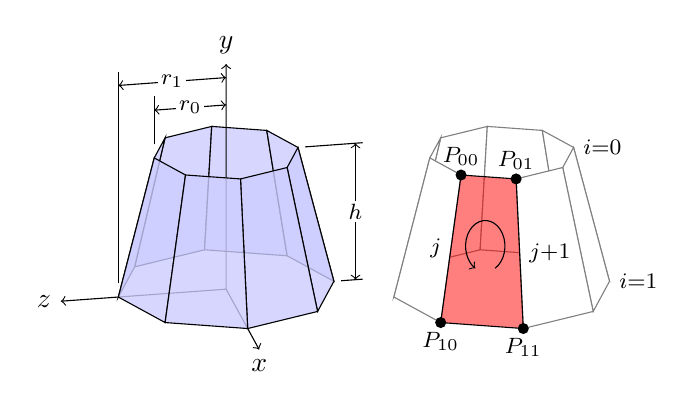
\begin{tikzpicture}
    \tikzstyle{conefill} = [fill=blue!20,fill opacity=0.8]
    \tikzstyle{ann} = [fill=white,font=\footnotesize,inner sep=1pt]
    \tikzstyle{ghostfill} = [fill=white]
    \tikzstyle{ghostdraw} = [draw=black!50]

    \filldraw[conefill](-.775,1.922)--(-1.162,.283)--(-.274,.5)
                        --(-.183,2.067)--cycle;
    \filldraw[conefill](-.183,2.067)--(-.274,.5)--(.775,.424)
                        --(.516,2.016)--cycle;
    \filldraw[conefill](.516,2.016)--(.775,.424)--(1.369,.1)
                        --(.913,1.8)--cycle;
    \filldraw[conefill](-.913,1.667)--(-1.369,-.1)--(-1.162,.283)
                        --(-.775,1.922)--cycle;
    \draw(1.461,.107)--(1.734,.127);
    \draw[arrows=<->](1.643,1.853)--(1.643,.12);
    \filldraw[conefill](.913,1.8)--(1.369,.1)--(1.162,-.283)
                        --(.775,1.545)--cycle;
    \draw[arrows=->,line width=.4pt](.274,-.5)--(0,0)--(0,2.86);
    \draw[arrows=-,line width=.4pt](0,0)--(-1.369,-.1);
    \draw[arrows=->,line width=.4pt](-1.369,-.1)--(-2.1,-.153);
    \filldraw[conefill](-.516,1.45)--(-.775,-.424)--(-1.369,-.1)
                        --(-.913,1.667)--cycle;
    \draw(-1.369,.073)--(-1.369,2.76);
    \draw(1.004,1.807)--(1.734,1.86);
    \filldraw[conefill](.775,1.545)--(1.162,-.283)--(.274,-.5)
                        --(.183,1.4)--cycle;
    \draw[arrows=<->](0,2.34)--(-.913,2.273);
    \draw(-.913,1.84)--(-.913,2.447);
    \draw[arrows=<->](0,2.687)--(-1.369,2.587);
    \filldraw[conefill](.183,1.4)--(.274,-.5)--(-.775,-.424)
                        --(-.516,1.45)--cycle;
    \draw[arrows=<-,line width=.4pt](.42,-.767)--(.274,-.5);
    \node[ann] at (-.456,2.307) {$r_0$};
    \node[ann] at (-.685,2.637) {$r_1$};
    \node[ann] at (1.643,.987) {$h$};
    \path (.42,-.767) node[below] {$x$}
        (0,2.86) node[above] {$y$}
        (-2.1,-.153) node[left] {$z$};
    % Second version of the cone
    \begin{scope}[xshift=3.5cm]
    \filldraw[ghostdraw,ghostfill](-.775,1.922)--(-1.162,.283)--(-.274,.5)
                                   --(-.183,2.067)--cycle;
    \filldraw[ghostdraw,ghostfill](-.183,2.067)--(-.274,.5)--(.775,.424)
                                   --(.516,2.016)--cycle;
    \filldraw[ghostdraw,ghostfill](.516,2.016)--(.775,.424)--(1.369,.1)
                                   --(.913,1.8)--cycle;
    \filldraw[ghostdraw,ghostfill](-.913,1.667)--(-1.369,-.1)--(-1.162,.283)
                                   --(-.775,1.922)--cycle;
    \filldraw[ghostdraw,ghostfill](.913,1.8)--(1.369,.1)--(1.162,-.283)
                                   --(.775,1.545)--cycle;
    \filldraw[ghostdraw,ghostfill](-.516,1.45)--(-.775,-.424)--(-1.369,-.1)
                                   --(-.913,1.667)--cycle;
    \filldraw[ghostdraw,ghostfill](.775,1.545)--(1.162,-.283)--(.274,-.5)
                                   --(.183,1.4)--cycle;
    \filldraw[fill=red,fill opacity=0.5](-.516,1.45)--(-.775,-.424)--(.274,-.5)
                                         --(.183,1.4)--cycle;
    \fill(-.775,-.424) circle (2pt);
    \fill(.274,-.5) circle (2pt);
    \fill(-.516,1.45) circle (2pt);
    \fill(.183,1.4) circle (2pt);
    \path[font=\footnotesize]
            (.913,1.8) node[right] {$i\hbox{$=$}0$}
            (1.369,.1) node[right] {$i\hbox{$=$}1$};
    \path[font=\footnotesize]
            (-.645,.513) node[left] {$j$}
            (.228,.45) node[right] {$j\hbox{$+$}1$};
    \draw (-.209,.482)+(-60:.25) [yscale=1.3,->] arc(-60:240:.25);
    \fill[black,font=\footnotesize]
                    (-.516,1.45) node [above] {$P_{00}$}
                    (-.775,-.424) node [below] {$P_{10}$}
                    (.183,1.4) node [above] {$P_{01}$}
                    (.274,-.5) node [below] {$P_{11}$};
    \end{scope}
\end{tikzpicture}

\marginpar{注释内容}

\newpage
\begin{table}
\caption{Timeline of something.}
\centering
\begin{minipage}[t]{.7\linewidth}
\color{gray}
\rule{\linewidth}{1pt}
\ytl{1947}{AT and T Bell Labs develop the idea of cellular phones}
\ytl{1968}{Xerox Palo Alto Research Centre envisage the `Dynabook'}
\ytl{1971}{Busicom 'Handy-LE' Calculator}
\ytl{1973}{First mobile handset invented by Martin Cooper}
\ytl{1978}{Parker Bros. Merlin Computer Toy}
\ytl{1981}{Osborne 1 Portable Computer}
\ytl{1982}{Grid Compass 1100 Clamshell Laptop}
\ytl{1983}{TRS-80 Model 100 Portable PC}
\ytl{1984}{Psion Organiser Handheld Computer}
\ytl{1991}{Psion Series 3 Minicomputer}
\bigskip
\rule{\linewidth}{1pt}%
\end{minipage}%
\end{table}

\newpage
$$
v = v^{1}e_{1} + v^{2}e_{2} + v^{3}e_{3} = v^{i}e_{i}, i = 1,2,3
$$

or 

\begin{equation}
v = v^{1}e_{1} + v^{2}e_{2} + v^{3}e_{3} = v^{i}e_{i}, i = 1,2,3
\end{equation}

$f(x) = \sum_{n=0}^{10} \frac{x}{n!}$  \\

$$
f(x) = \sum_{n=0}^{10} \frac{x}{n!}
$$

In-line math components can be set with independent math display style 
$f(x) = \displaystyle \sum_{n=0}^{10} \frac{x}{n!}$, and vice versa:
$$
f(x) = \scriptstyle \sum_{n=0}^{10} \frac{x}{n!}
$$


\begin{equation}\label{eq:Pythagorean theorem}
x^{2}+y^{2}=z^{2}
\end{equation}
公式\ref{eq:Pythagorean theorem}是毕达哥拉斯定理,在中国又称勾股定理。

$$
\mbox{例如:} x_{1}, x_{2}, \cdots, x_{N} 
$$ 

$$
\left [
\begin{array}{cc}
v^{i} e_{i} & v^{i} e_{j}  \\
v^{j} e_{i} & v^{j} e_{j}  \\
\end{array}
\right ]
$$

$$
\left \{
\begin{array}{r c l}
(f + g)(x)    & = &  f(x) + g(x) \\
(\alpha f)(x) & = &  \alpha f(x) \\
(fg)(x)       & = &  f(x)g(x)    \\
\end{array}
\right .
$$

在这里添加页脚注释角标\footnotemark
%% ...
在这里设置注释内容\footnotetext{注释内容}

正文内容\footnote{注释内容\label{fnote}}
在这里也引用与上边脚注相同的角标 \textsuperscript{\ref{fnote}}


\newpage
\begin{eqnarray} 
w(0) & = & 0 \\
\frac{\partial w}{\partial x}\Big |_{x=0} & = & 0  \\
\end{eqnarray}


$$ s = \int_{a}^{b} |\dot{x}(t)| dt  $$

$$ r'(t) = \lim \limits_{\triangle t \rightarrow 0} \frac{ r(t + \triangle t) - r(t)}{ \triangle t }$$

$$
\frac{\partial w}{\partial x}\Big |_{x=0} = 0 
$$

The square root of 100 is $\sqrt{100}=10$. 
\\
The cubic root of 64 is $\sqrt[3]{64}=4$.

\footnote{注释内容}



\newpage
 \begin{thebibliography}{9}
\bibitem{latexcompanion} 
Helmut Kopka and Patrick W. Daly. 
\textit{A Guide to \LaTeX\ }. 
Addison-Wesley, Fourth edition, 2004.


\bibitem{latexcompanion} 
Michel Goossens, Frank Mittelbach, and Alexander Samarin. 
\textit{The \LaTeX\ Companion}. 
Addison-Wesley, Reading, Massachusetts, 1993.
 
\bibitem{einstein} 
Albert Einstein. 
\textit{Zur Elektrodynamik bewegter K{\"o}rper}. (German) 
[\textit{On the electrodynamics of moving bodies}]. 
Annalen der Physik, 322(10):891–921, 1905.
 

\newpage
\begin{equation}       %开始数学环境
\left(                 %左括号
  \begin{array}{ccc}   %该矩阵一共3列,每一列都居中放置
    a11 & a12 & a13\\  %第一行元素
    a21 & a22 & a23\\  %第二行元素
  \end{array}
\right)                 %右括号
\end{equation}


%% 通常可以用\bordermatrix 来实现: 给矩阵行和列有个说明或者编号
$\bordermatrix{%
& 1 & 2 \cr
1 & x1 & x2 \cr
2 & x3 & x4 \cr
3 & x5 & x6
}$

%% 使用blkarray 宏包来实现:给矩阵行和列有个说明或者编号

\newpage
\begin{equation}       %开始数学环境
\left(                 %左括号
  \begin{array}{cccc}   %该矩阵一共3列,每一列都居中放置
    1 & -2 & 1  & 0 \\  %
    0 & 1 & -4 & 4 \\ %
    0 & 0 & 1 & 3 \\  %
  \end{array}
\right)                 %右括号
\end{equation}

\begin{equation}       %开始数学环境
\left(                 %左括号
  \begin{array}{cccc}   %该矩阵一共3列,每一列都居中放置
    0 & 1 & -4 & 8 \\  %
    2 & -3 & 2 & 1 \\ %
    5 & -8 & 7 & 1 \\  %
  \end{array}
\right)                 %右括号
\end{equation}


\newpage
\newpage
\newpage
\newpage
\newpage
\newpage
\newpage
\newpage
\newpage
\newpage
\newpage

\newpage
\bibitem{knuthwebsite} 
Knuth: Computers and Typesetting,
\\\texttt{http://www-cs-faculty.stanford.edu/\~{}uno/abcde.html}
\end{thebibliography}


\end{document} 